\documentclass[11pt]{article}

\usepackage[utf8]{inputenc}
\usepackage[T1]{fontenc}
\usepackage{indentfirst}
\usepackage{titlesec}
\usepackage{listings}
\usepackage{float}

\titlelabel{\thetitle.\quad}

\renewcommand{\lstlistingname}{Programski odsječak}
\renewcommand{\figurename}{Slika}
\renewcommand{\tablename}{Tablica}

%Gummi|063|=)
\title{\textbf{PDQ - Analiza performansi}\\
		Raspodijeljeni sustavi - 3. domaća zadaća}
\author{Matija Šantl \\
		0036458898}
\date{}
\usepackage{graphicx}
\begin{document}

\maketitle

\section{Zadatak}
Web aplikacija uključuje podršku korisnicima putem usluge za \emph{chat}. Kupci sami odabiru jedan od 10 repova čekanja u kojima upite poslužuje po jedan tehničar. Mjerenja pokazuju da zahtjevi prosječno dolaze 3 upita u minuti te da svaki kupac prosječno čeka 3 minute u repu i prosječno provodi 2 minute u razgovoru.

\subsection{Kakvi će biti odazivi sa 10 osoba - poslužitelja ako publiciranje Web-stranice sa odgovorima na najčešća pitanja smanji broj upita na 2 u minuti ?}

$N =10$

$L = 2 upit / min$

$S = 2 min / upit$

$U_a = L \cdot S = 2 \cdot 2 = 4$

$\rho = \frac{U}{N} = \frac{4}{10} = 0.4$

$R = \frac{S}{1 - \rho} = \frac{2}{0.6} = 3.333 min / upit$

$W = R - S = 3.333 - 2 = 1.333 min / upit$

Vrijeme čekanja se smanjilo smanjenjem broja upita u minuti. 

\subsection{Kakvi će biti odazivi sa 18 osoba - poslužitelja ako publiciranje Web-stranice sa odgovorima na najčešća pitanja smanji broj upita na 2 u minuti ?}

$N =18$

$L = 2 upit / min$

$S = 2 min / upit$

$U_a = L \cdot S = 2 \cdot 2 = 4$

$\rho = \frac{U}{N} = \frac{4}{18} = 0.222$

$R = \frac{S}{1 - \rho} = \frac{2}{0.778} = 2.571 min / upit$

$W = R - S = 2.571 - 2 = 0.571 min / upit$

Vrijeme čekanja se smanjilo smanjenjem broja upita u minuti, a dodatno smanjenje vremena čekanja je uzrokovano povećanjem broja poslužitelja.

\subsection{Kakve će rezultate dati smanjenje razgovora na 1.5 minutu ? (N = 10)}

$N =10$

$L = 3 upit / min$

$S = 1.5 min / upit$

$U_a = L \cdot S = 3 \cdot 1.5 = 4.5$

$\rho = \frac{U}{N} = \frac{4.5}{10} = 0.45$

$R = \frac{S}{1 - \rho} = \frac{1.5}{0.55} = 2.727 min / upit$

$W = R - S = 2.727 - 1.5 = 1.227 min / upit$

Vrijeme čekanja se smanjilo smanjenjem vremena posluživanja zahtjeva,

\subsection{Kakve će rezultate dati smanjenje razgovora na 1.5 minutu ? (N = 18)}

$N =18$

$L = 3 upit / min$

$S = 1.5 min / upit$

$U_a = L \cdot S = 3 \cdot 1.5 = 4.5$

$\rho = \frac{U}{N} = \frac{4.5}{18} = 0.25$

$R = \frac{S}{1 - \rho} = \frac{1.5}{0.75} = 2 min / upit$

$W = R - S = 2 - 1.5 = 0.5 min / upit$

Vrijeme čekanja se smanjilo smanjenjem vremena posluživanja zahtjeva, a dodtano smanjenje vremena čekanja je uzrokovano povečanjem broja poslužitelja.

\section{Zadatak}
Oblikovati proizvoljnu raspodijeljenu aplikaciju i ostvariti analizu performansi ostvarene aplikacije.

\newpage

\subsection{Definirati logičku i fizičku arhitekturu aplikacije}

\begin{figure}[h!]
	\caption{Logička arhitektura.}
	\centering
	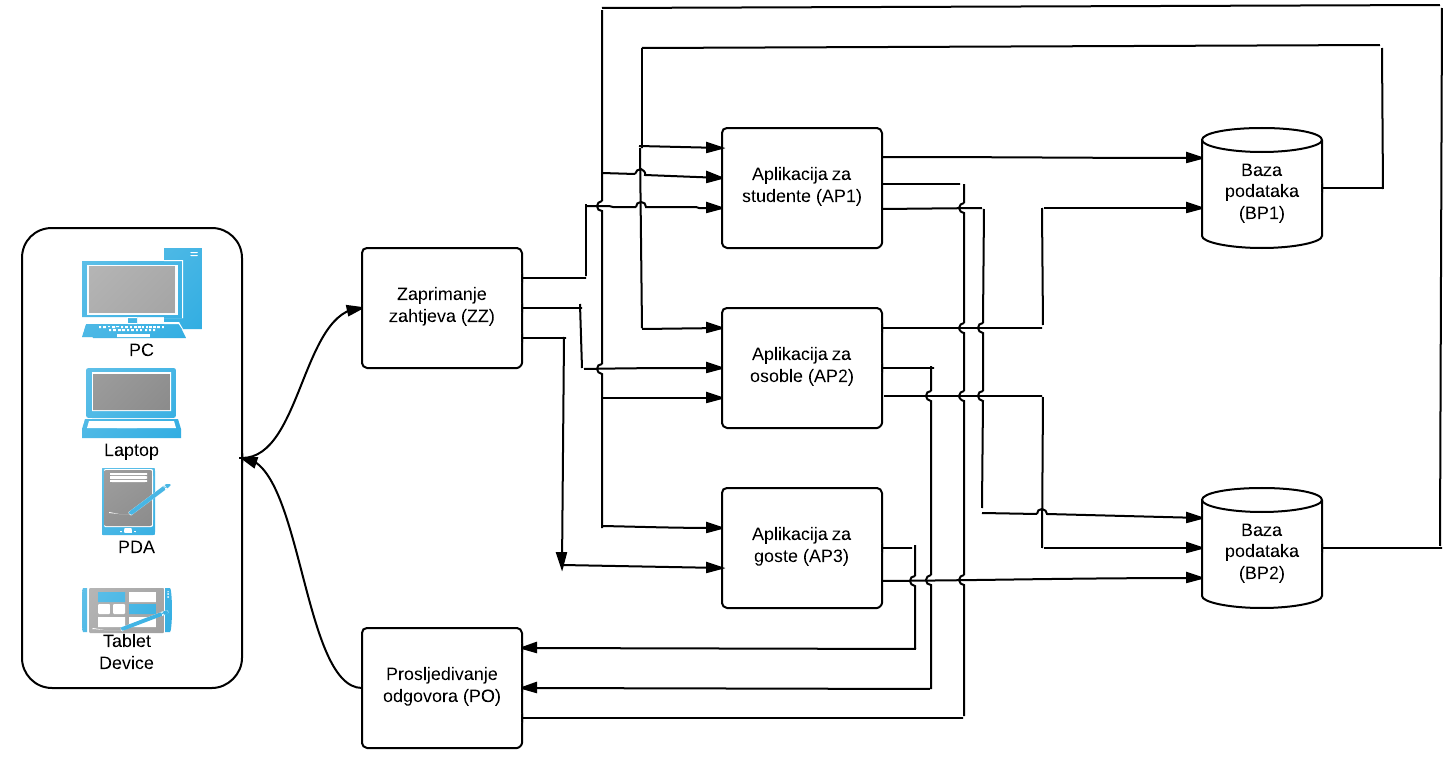
\includegraphics[width=1.3\textwidth,angle=90]{logicka.png}
\end{figure}

\newpage

\begin{figure}[h!]
	\caption{Fizička arhitektura.}
	\centering
	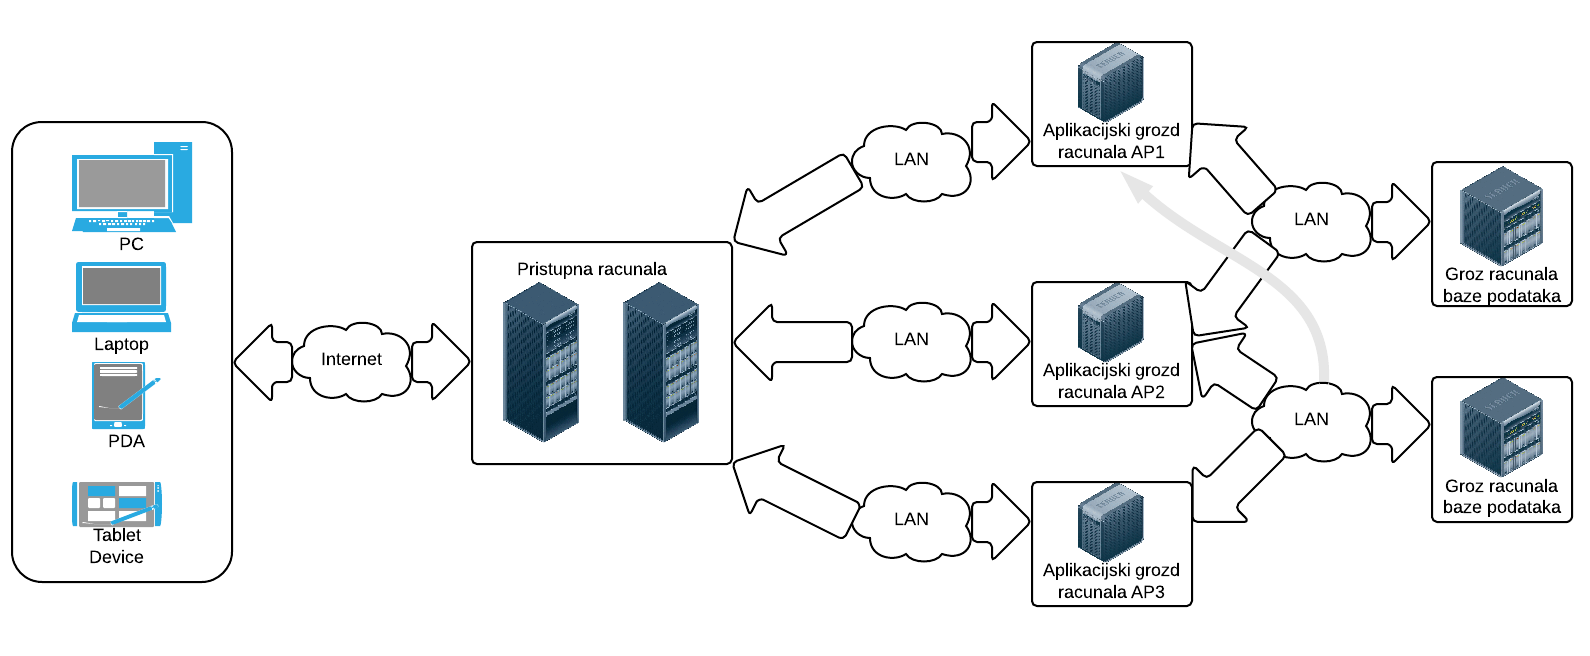
\includegraphics[width=1.3\textwidth,angle=90]{fizicka.png}
\end{figure}

\subsection{Izgraditi model aplikacije primjenom teorije repova}
Odrediti analitičko rješenje funkcije zadržavanja zahtjeva u aplikaciji $R = f(L)$

\begin{figure}[h!]
	\caption{Model aplikacije}
	\centering
	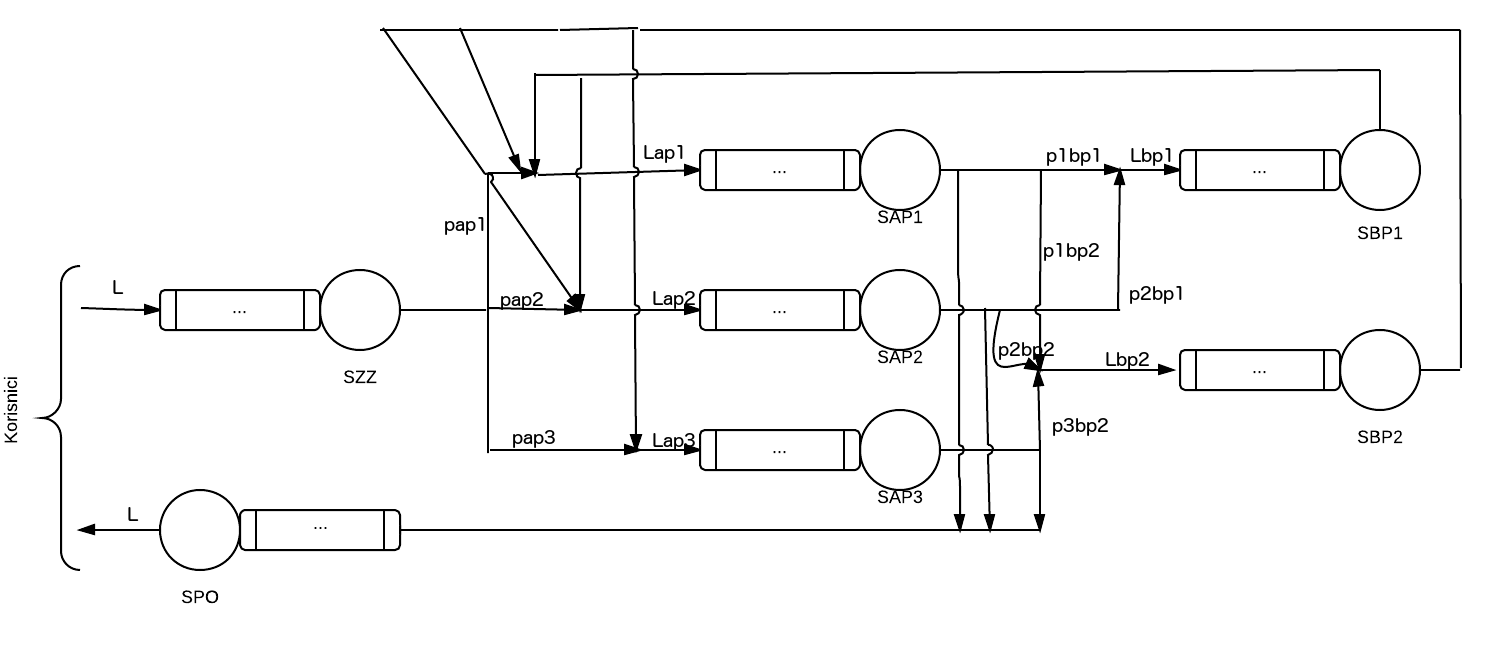
\includegraphics[width=1.2\textwidth,angle=90]{model.png}
\end{figure}

\newpage

Analiza primjenom teorije repova je dana u nastavku.

$L_{ZZ} = L$ i $L_{PO} = L$
\vspace{10px}

$L_{AP1} = p_{1BP1} \cdot L_{AP1} + p_{1BP2} \cdot L_{AP1} + p_{AP1} \cdot L $
\vspace{10px}

$L_{AP1} = \frac{p_{AP1}}{1 - (p_{1BP1} + p_{1BP2})} \cdot L$
\vspace{10px}

$L_{AP2} = p_{2BP1} \cdot L_{AP2} + p_{2BP2} \cdot L_{AP2} + p_{AP2} \cdot L $
\vspace{10px}

$L_{AP2} = \frac{p_{AP2}}{1 - (p_{2BP1} + p_{2BP2})} \cdot L$
\vspace{10px}

$L_{AP3} = p_{3BP2} \cdot L_{AP3} + p_{AP3} \cdot L $
\vspace{10px}

$L_{AP3} = \frac{p_{AP3}}{1 - p_{3BP2}} \cdot L$
\vspace{10px}

$L_{BP1} = p_{BP1} \cdot L_{AP1} + p_{2BP1} \cdot L_{AP2}$
\vspace{10px}

$L_{BP1} = (p_{1BP1} \cdot \frac{p_{AP1}}{1 - (p_{1BP1} + p_{1BP2} )} + p_{2BP1} \cdot \frac{p_{AP2}}{1 - (p_{2BP1} + p_{2BP2})}) \cdot L$
\vspace{10px}

$L_{BP2} = p_{BP2} \cdot L_{AP1} + p_{2BP2} \cdot L_{AP2} + p_{3BP2} \cdot L_{AP3}$
\vspace{10px}

$L_{BP2} = (p_{1BP2} \cdot \frac{p_{AP1}}{1 - (p_{1BP1} + p_{1BP2} )} + p_{2BP2} \cdot \frac{p_{AP2}}{1 - (p_{2BP1} + p_{2BP2})} + p_{3BP2 \cdot \frac{p_{AP3}}{1-p_{3BP2}}}) \cdot L$
\vspace{10px}

Iz izraza za intenzitet dolazaka možemo isčitati vrijednosti $v_x$ koje nam trebaju za izračun prosječnog vremena zadržavanja, $R$. 
Tako redom imamo:

$v_{AP1} = \frac{p_{AP1}}{1 - (p_{1BP1} + p_{1BP2})}$
\vspace{10px}

$v_{AP2} = \frac{p_{AP2}}{1 - (p_{2BP1} + p_{2BP2})}$
\vspace{10px}

$v_{AP3} = \frac{p_{AP3}}{1 - p_{3BP2}}$
\vspace{10px}

$v_{BP1} = p_{1BP1} \cdot \frac{p_{AP1}}{1 - (p_{1BP1} + p_{1BP2} )} + p_{2BP1} \cdot \frac{p_{AP2}}{1 - (p_{2BP1} + p_{2BP2})}$
\vspace{10px}

$v_{BP2} = p_{1BP2} \cdot \frac{p_{AP1}}{1 - (p_{1BP1} + p_{1BP2} )} + p_{2BP2} \cdot \frac{p_{AP2}}{1 - (p_{2BP1} + p_{2BP2})} + p_{3BP2 \cdot \frac{p_{AP3}}{1-p_{3BP2}}}$
\vspace{10px}

$v_{ZZ} = 1$
\vspace{10px}

$v_{PO} = 1$
\vspace{10px}

Izraz za prosječno vrijeme zadržavanja glasi:
$ R = \sum_{i} v_i \cdot R_i $
\vspace{10px}

pri čemu se umnožak $v_i \cdot R_i$ može zapisati kao

$v_i \cdot R_i = \frac{v_i \cdot S_i}{1 - U_i} = \frac{v_i \cdot S_i}{1 - v_i \cdot L \cdot S_i} = \frac{D_i}{1 - L \cdot D_i} $
\vspace{10px}

Vrijednosti $D$ računamo na sljedeći način:
\vspace{10px}

$D_{ZZ} = S_{ZZ}$
\vspace{10px}

$D_{PO} = S_{PO}$
\vspace{10px}

$D_{AP1} = v_{AP1} \cdot S_{AP}$
\vspace{10px}

$D_{AP2} = v_{AP2} \cdot S_{AP}$
\vspace{10px}

$D_{AP3} = v_{AP3} \cdot S_{AP}$
\vspace{10px}

$D_{BP1} = v_{BP1} \cdot S_{BP}$
\vspace{10px}

$D_{BP2} = v_{BP2} \cdot S_{BP}$
\vspace{10px}

Konačni izraz za vrijednost $R$ izgleda ovako:
\vspace{10px}

$R = \frac{D_{ZZ}}{1 - L \cdot D_{ZZ}} + \frac{D_{PO}}{1 - L \cdot D_{PO}} + \frac{D_{AP1}}{1 - L \cdot D_{AP1}} + \frac{D_{AP2}}{1 - L \cdot D_{AP2}} + \frac{D_{AP3}}{1 - L \cdot D_{AP3}} + \frac{D_{BP1}}{1 - L \cdot D_{BP1}} + \frac{D_{BP2}}{1 - L \cdot D_{BP2}} $

\vspace{10px}

Vrijednosti koje su korištene prilikom računanja su sljedeće:

$ p_{AP1} = 0.2 $, $ p_{AP2} = 0.3 $, $ p_{AP3} = 0.5 $

$ p1_{BP1} = 0.1 $, $ p1_{BP2} = 0.3 $

$ p2_{BP1} = 0.3 $, $ p2_{BP2} = 0.1 $

$ p3_{BP2} = 0.1 $

$ S_{ZZ} = 0.001 $, $ S_{PO} = 0.001 $

$ S_{AP} = 0.3 $, $ S_{BP} = 4.5 $

\begin{table}[h!]
  \begin{center}
    \begin{tabular}{| c c c c c c c c c |}
    \hline
L    & AP1 & AP2 & AP3 & BP1 & BP2 & ZZ & PO & R \\
0.2 & 0.102 & 0.155 & 0.172 & 0.988 & 1.135 & 0.001 & 0.001 & 2.554\\
0.4 & 0.104 & 0.160 & 0.179 & 1.231 & 1.468 & 0.001 & 0.001 & 3.144\\
0.6 & 0.106 & 0.165 & 0.185 & 1.634 & 2.079 & 0.001 & 0.001 & 4.171\\
0.8 & 0.109 & 0.170 & 0.192 & 2.426 & 3.558 & 0.001 & 0.001 & 6.457\\
1 & 0.111 & 0.176 & 0.200 & 4.714 & 12.333 & 0.001 & 0.001 & 17.536\\

    \hline
    \end{tabular}
  \end{center}
  \caption{Rezultati dobiveni analitičkim putem}
\end{table}

\subsection{Izgraditi model aplikacije za alat \emph{PDQ}}
Primjenom izgrađenog modela ostvariti vrijednosti funkcije zadržavanja zahtjeva $R = f(L)$ u nekoliko točaka.

Kao implementacijski jezik za ostvarivanje modela u alatu \emph{PDQ} odabrao sam programski jezik \emph{R}.  

\begin{table}[h!]
  \begin{center}
    \begin{tabular}{| c c c c c c c c c |}
    \hline
L & AP1 & AP2 & AP3 & BP1 & BP2 & ZZ & PO & R \\
0.04 & 0.100 & 0.151 & 0.168 & 0.853 & 0.961 & 0.001 & 0.001 & 2.235\\
0.08 & 0.101 & 0.152 & 0.169 & 0.883 & 0.999 & 0.001 & 0.001 & 2.306\\
0.12 & 0.101 & 0.153 & 0.170 & 0.916 & 1.040 & 0.001 & 0.001 & 2.382\\
0.16 & 0.102 & 0.154 & 0.171 & 0.950 & 1.086 & 0.001 & 0.001 & 2.465\\
0.2 & 0.102 & 0.155 & 0.172 & 0.988 & 1.135 & 0.001 & 0.001 & 2.554\\
0.24 & 0.102 & 0.156 & 0.174 & 1.029 & 1.189 & 0.001 & 0.001 & 2.651\\
0.28 & 0.103 & 0.157 & 0.175 & 1.073 & 1.248 & 0.001 & 0.001 & 2.757\\
0.32 & 0.103 & 0.158 & 0.176 & 1.121 & 1.314 & 0.001 & 0.001 & 2.874\\
0.36 & 0.104 & 0.159 & 0.177 & 1.174 & 1.387 & 0.001 & 0.001 & 3.002\\
0.4 & 0.104 & 0.160 & 0.179 & 1.231 & 1.468 & 0.001 & 0.001 & 3.144\\
0.44 & 0.105 & 0.161 & 0.180 & 1.295 & 1.560 & 0.001 & 0.001 & 3.302\\
0.48 & 0.105 & 0.162 & 0.181 & 1.366 & 1.664 & 0.001 & 0.001 & 3.479\\
0.52 & 0.105 & 0.163 & 0.182 & 1.445 & 1.782 & 0.001 & 0.001 & 3.680\\
0.56 & 0.106 & 0.164 & 0.184 & 1.533 & 1.919 & 0.001 & 0.001 & 3.908\\
0.6 & 0.106 & 0.165 & 0.185 & 1.634 & 2.079 & 0.001 & 0.001 & 4.171\\
0.64 & 0.107 & 0.166 & 0.187 & 1.748 & 2.267 & 0.001 & 0.001 & 4.476\\
0.68 & 0.107 & 0.167 & 0.188 & 1.879 & 2.493 & 0.001 & 0.001 & 4.837\\
0.72 & 0.108 & 0.168 & 0.189 & 2.032 & 2.769 & 0.001 & 0.001 & 5.269\\
0.76 & 0.108 & 0.169 & 0.191 & 2.212 & 3.114 & 0.001 & 0.001 & 5.797\\
0.8 & 0.109 & 0.170 & 0.192 & 2.426 & 3.558 & 0.001 & 0.001 & 6.458\\
0.84 & 0.109 & 0.172 & 0.194 & 2.687 & 4.148 & 0.001 & 0.001 & 7.312\\
0.88 & 0.110 & 0.173 & 0.195 & 3.011 & 4.973 & 0.001 & 0.001 & 8.464\\
0.92 & 0.110 & 0.174 & 0.197 & 3.423 & 6.208 & 0.001 & 0.001 & 10.114\\
0.96 & 0.111 & 0.175 & 0.198 & 3.966 & 8.259 & 0.001 & 0.001 & 12.712\\
1 & 0.111 & 0.176 & 0.200 & 4.714 & 12.333 & 0.001 & 0.001 & 17.537\\
1.04 & 0.112 & 0.178 & 0.202 & 5.810 & 24.342 & 0.001 & 0.001 & 30.645\\
1.08 & 0.112 & 0.179 & 0.203 & 7.569 & 925.000 & 0.001 & 0.001 & 933.065\\
    \hline
    \end{tabular}
  \end{center}
  \caption{Rezultati dobiveni programskim putem}
\end{table}


\begin{figure}[h!]
	\caption{Vrijeme zadržavanja zahtjeva u sustavu}
	\centering
	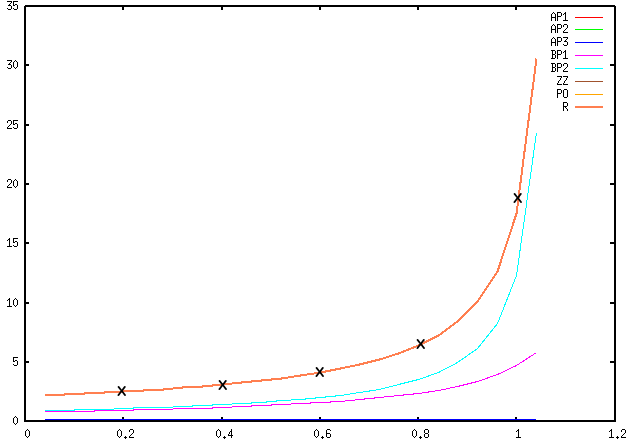
\includegraphics[width=1.2\textwidth]{graf.png}
\end{figure}

Izvorni kod korišten za simulaciju u alatu \emph{PDQ} se nalazi u Dodatku A.

\subsection{Usporediti i obrazložiti dobivene rezultate}

Rezultati dobiveni uvrštavanjem vrijednosti korištenih u simulaciji alatom \emph{PDQ} u izraz dobiven primjenom teorije repova na model aplikacje su identični na 3 decimale. Iz toga možemo zaključiti kako je \emph{PDQ} model ispravno zadan i izveden. 

Prema dobivenim rezultatima za odabrani raspodijeljeni sustav zaključujem kako on uz odabrane parametre prihvatljivo funkcionira do trenutka kada učestalost zahtjeva ne pređe iznos $0.8 zahtjev / sekundi $. Nakon toga, pa sve do iznosa $1.09 zahtjev / sekundi$ performanse eskponencijalno degradiraju, te u tom području sustav postaje prezasićen.

Kada bismo htjeci povećati propusnost i omogućiti rad pri većim opterećenjima, sustav je potrebno nadograditi.


\newpage

\appendix
\section{PDQ - izvorni kod} \label{Dodatak A}

\begin{lstlisting}[caption=Izvorni kod u jeziku R, label=pdq_r, language=R, numbers=left]
library(pdq)

# udio ulaza koji odlazi na ap1
p_ap1 = 0.2
# udio ulaza koji odlazi na ap2
p_ap2 = 0.3
# udio ulaza koji odlazi na ap3
p_ap3 = 0.5

# udio izlaza ap1 koji odlazi na bp1
p1_bp1 = 0.1
# udio izlaza ap1 koji odlazi na bp2
p1_bp2 = 0.3

# udio izlaza ap2 koji odlazi na bp1
p2_bp1 = 0.3
# udio izlaza ap2 koji odlazi na bp2
p2_bp2 = 0.1

# udio izlaza ap3 koji odlazi na bp2
p3_bp2 = 0.1

# ulaz
S_ZZ = 0.001
# izlaz
S_PO = 0.001

# svi aplikacijski grozdovi su jednaki
S_AP = 0.3
# sve baze podataka su jednake
S_BP = 4.5

# apsolutne vrijednosti udjela
v_ap1 = p_ap1 / (1 - p1_bp1 - p1_bp2)
v_ap2 = p_ap2 / (1 - p2_bp1 - p2_bp2)
v_ap3 = p_ap3 / (1 - p3_bp2)

v_bp1 = p1_bp1 * v_ap1 + p2_bp1 * v_ap2
v_bp2 = p1_bp2 * v_ap1 + p2_bp2 * v_ap2 + p3_bp2 * v_ap3

# print(c(v_ap1, v_ap2, v_ap3, v_bp1, v_bp2))

# domena
L_inc = 0.04
L_start = L_inc
L_end = 1.08

# solve for various L's 
for (L in seq(L_start, L_end, by=L_inc)) {
	Init("RASSUS - 3.dz")
	
	CreateOpen("Zahtjevi", L)
	
	SetWUnit("Zahtjevi")
	SetTUnit("Sec")
	
	# create nodes
	CreateNode("ZZ", CEN, FCFS)
	CreateNode("PO", CEN, FCFS)
	
	CreateNode("AP1", CEN, FCFS)
	CreateNode("AP2", CEN, FCFS)
	CreateNode("AP3", CEN, FCFS)
	
	CreateNode("BP1", CEN, FCFS)
	CreateNode("BP2", CEN, FCFS)
	
	# connect them
	SetVisits("ZZ", "Zahtjevi", 1.0, S_ZZ)
	SetVisits("PO", "Zahtjevi", 1.0, S_PO)
	
	SetVisits("AP1", "Zahtjevi", v_ap1, S_AP)
	SetVisits("AP2", "Zahtjevi", v_ap2, S_AP)
	SetVisits("AP3", "Zahtjevi", v_ap3, S_AP)	
	
	SetVisits("BP1", "Zahtjevi", v_bp1, S_BP)
	SetVisits("BP2", "Zahtjevi", v_bp2, S_BP)

	# pdq magic
	Solve(CANON)	
	
	# prepare results
	response = sprintf("%.3f", 
		GetResponse(TRANS, "Zahtjevi"))
	
	t_ap1 = sprintf("%.3f", 
		GetResidenceTime("AP1", "Zahtjevi", TRANS))
	t_ap2 = sprintf("%.3f", 
		GetResidenceTime("AP2", "Zahtjevi", TRANS))
	t_ap3 = sprintf("%.3f", 
		GetResidenceTime("AP3", "Zahtjevi", TRANS))
	
	t_bp1 = sprintf("%.3f", 
		GetResidenceTime("BP1", "Zahtjevi", TRANS))
	t_bp2 = sprintf("%.3f", 
		GetResidenceTime("BP2", "Zahtjevi", TRANS))
	
	t_zz = sprintf("%.3f", 
		GetResidenceTime("ZZ", "Zahtjevi", TRANS))
	t_po = sprintf("%.3f", 
		GetResidenceTime("PO", "Zahtjevi", TRANS))
	
	l = sprintf("%.3f", L)
	
	result <- c(L, t_ap1, t_ap2, t_ap3, 
			t_bp1, t_bp2, t_zz, t_po, response)
	
	print(result)
	
	# Report()
}
\end{lstlisting}

\newpage

\begin{figure}[h!]
	\caption{Primjer izvođenja izvornog koda}
	\centering
	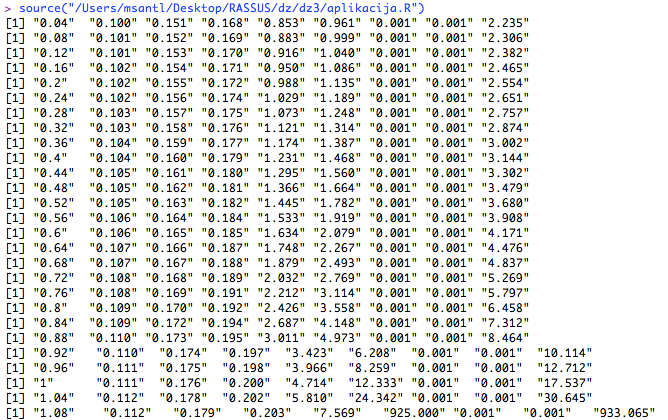
\includegraphics[width=1.3\textwidth]{izvodjenje.png}
\end{figure}

\end{document}
